 
  \documentclass[final]{beamer} % beamer 3.10: do NOT use option hyperref={pdfpagelabels=false} !

  %\documentclass[final,hyperref={pdfpagelabels=false}]{beamer} % beamer 3.07: get rid of beamer warnings
  \mode<presentation> {  %% check http://www-i6.informatik.rwth-aachen.de/~dreuw/latexbeamerposter.php for examples
    \usetheme{Berlin}    %% you should define your own theme e.g. for big headlines using your own logos 
  }
\setbeamercolor{block body}{bg=white, fg=black}
\setbeamerfont{block title}{size=\Large}
  \usepackage[english]{babel}
  \usepackage[latin1]{inputenc}
  \usepackage{amsmath,amsthm, amssymb, latexsym}
  \usepackage{float}
  \usepackage{booktabs}
\usepackage{mathptmx}
\usepackage{color}
\usepackage{pgfplots}
\usepackage{anyfontsize}
  %\usepackage{times}\usefonttheme{professionalfonts}  % times is obsolete
  \usefonttheme[onlymath]{serif}
  \boldmath
  \usepackage[orientation=portrait,size=a0,scale=1.10, debug]{beamerposter}                       % e.g. for DIN-A0 poster
  %\usepackage[orientation=portrait,size=a1,scale=1.4,grid,debug]{beamerposter}                  % e.g. for DIN-A1 poster, with optional grid and debug output
  %\usepackage[size=custom,width=200,height=120,scale=2,debug]{beamerposter}                     % e.g. for custom size poster
  %\usepackage[orientation=portrait,size=a0,scale=1.0,printer=rwth-glossy-uv.df]{beamerposter}   % e.g. for DIN-A0 poster with rwth-glossy-uv printer check
  % ...
\definecolor{OliveGreen}{HTML}{eeeeee}

\begin{document}

  \begin{frame}
    \begin{center}

      \textcolor{black}{
      \textbf{\fontsize{110}{200}{\selectfont Panthera: A Study of Caching in }}
      \vspace{0.5em}
      \textbf{\fontsize{110}{200}{\selectfont Distributed Computing}}}
    \end{center}
    
    \begin{columns}[t]
     \begin{column}{0.32\textwidth}
      \begin{block}{Background}
      \textbf{Distributed computing} has seen tremendous growth in the past few years. 
      Essentially, \textbf{it allows computational algorithms to run across multiple
      computers (i.e. nodes)}. Most distributed systems must make files accessible over 	networks of computers. \textbf{This 
      project aims to reduce the waiting time (known as \textit{latency}) associated
      with obtaining files within distributed computing systems}.
      \end{block}
      \begin{block}{Introduction}
      Hadoop, an open source project that allows developers to
write distributed applications, has found extensive use in academia and industry. For example, Yahoo, Facebook, Stanford Computer Science, etc. are all heavily involved with Hadoop development. But, Hadoop does not effectively utilize Random Access Memory (RAM) and local storage to better performance. \textbf{This project develops and tests scheduling and caching mechanisms to reduce waiting time (i.e. latency) in Hadoop, thereby greatly increasing Hadoop's efficiency and applicability in fields ranging from medical diagnosis to artificial intelligence.}
      \end{block}

	\begin{block}{Caching}
	There is significant waiting time/latency associated with retrieving files from distributed filesystems (Griffioen 1994). \textbf{Caches} are used to store
	some files locally so that they can be accessed much more quickly. Panthera implements a cache and a cache-based scheduler for Hadoop.
	\end{block}
	
    \begin{block}{Problem}
	\begin{itemize}
	 \item \textbf{Develop a caching layer} for the Hadoop Distributed File System that can cache \textbf{both data and metadata}.
	 \item The solution should be a \textbf{"drop-in" addition}, allowing for easy adoption and integration into existing systems.
	 \item The layer \textbf{should reduce file access latency}/waiting time significantly in comparison to \textbf{the control group: a standard Hadoop installation}.
	 \item \textbf{Develop a scheduler} for the Hadoop which \textbf{schedules jobs based on what is available in the cache}. In addition, it should be be able to \textbf{prefetch files that could be needed in the future}.
	\end{itemize}

      \end{block}

      \begin{block}{Hypothesis}
       The cache layer designed (called \textbf{Panthera}) will have lower file
       access latency when compared to a standard Hadoop installation. Additionally, it
       will be possible to design \textbf{Panthera} such that the Hadoop source code
       remains unaffected. It will also be feasible to create a cache-based 
       scheduler for Hadoop.
      \end{block}
	  
		\begin{block}{Data vs Metadata}
			\textbf{Data} within the Hadoop file system \textbf{consists of the actual contents of a file.}
			\textbf{Metadata is the information about files and directories}, e.g. time a file was created, the list of files in a directory, etc. \textbf{Panthera performs both metadata
			and data caching; both have significantly different technical implications
			and challenges.}
		\end{block}
	
		\begin{block}{Current Hadoop File System Architecture}
			\centerline{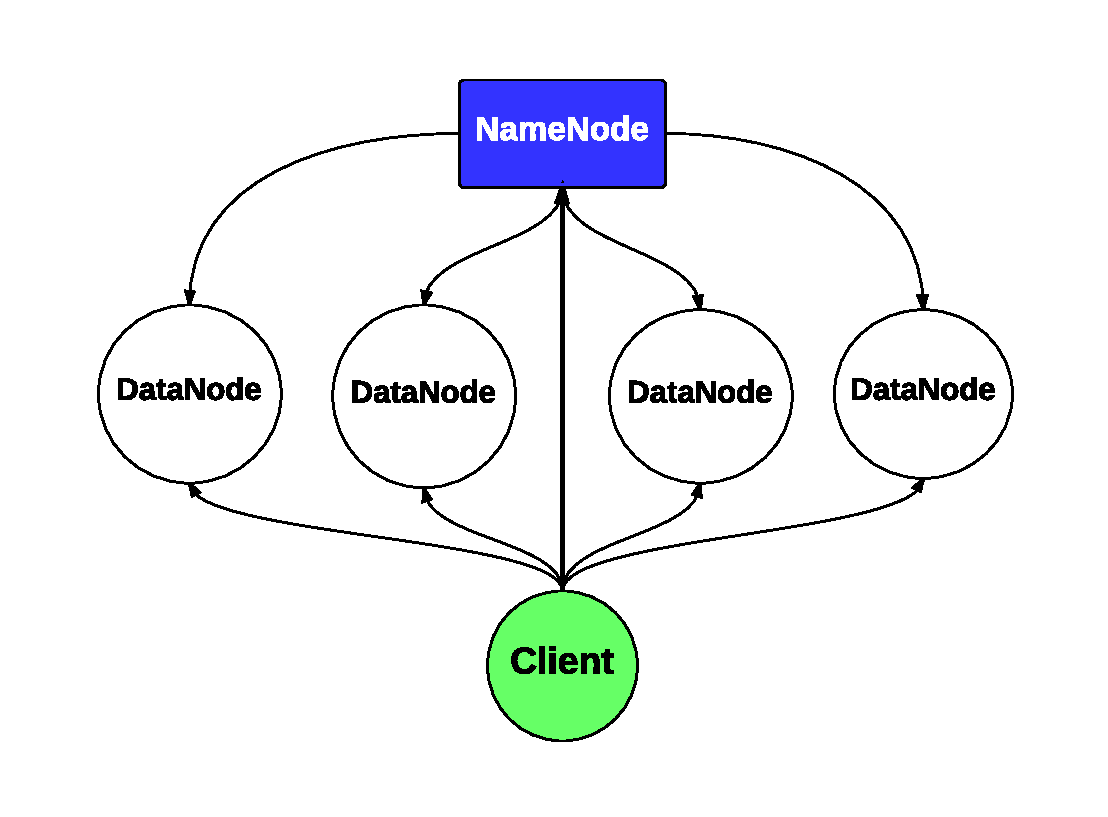
\includegraphics[scale=1.5]{assets/vanilla_hadoop.pdf}}
		\end{block}
		
	  

     \end{column}
     %##########################################################################################################

    \begin{column}{0.32\textwidth}
		\begin{block}{Panthera Architecture}
		\vspace{1em}
		\centerline{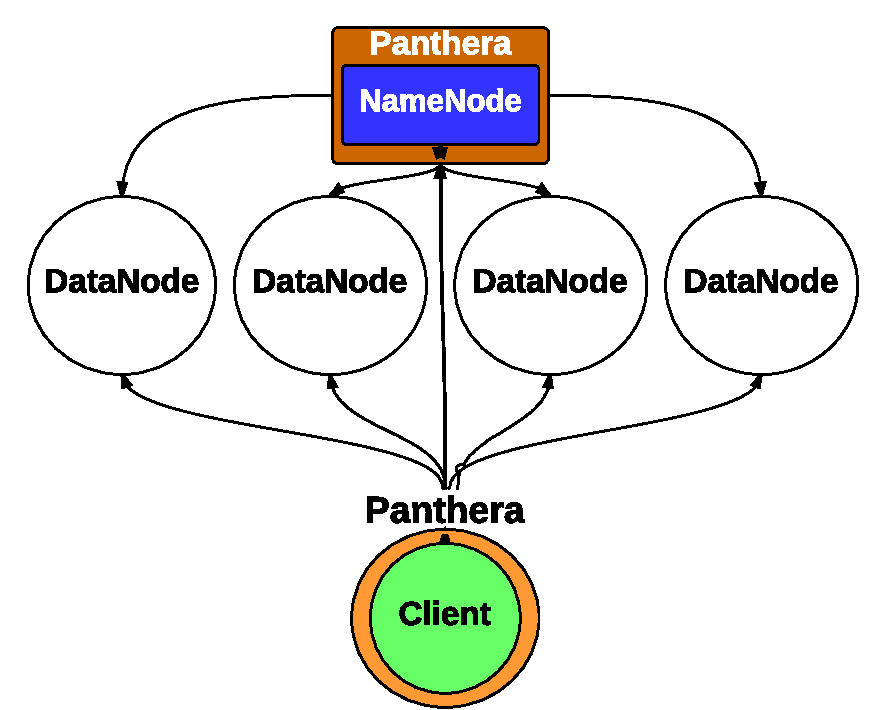
\includegraphics[scale=1.5]{assets/v2/panthera_hadoop_arch.pdf}}	  
	  \end{block}   	  
		%\begin{block}{Panthera Metadata Architecture}
	 		%\centerline{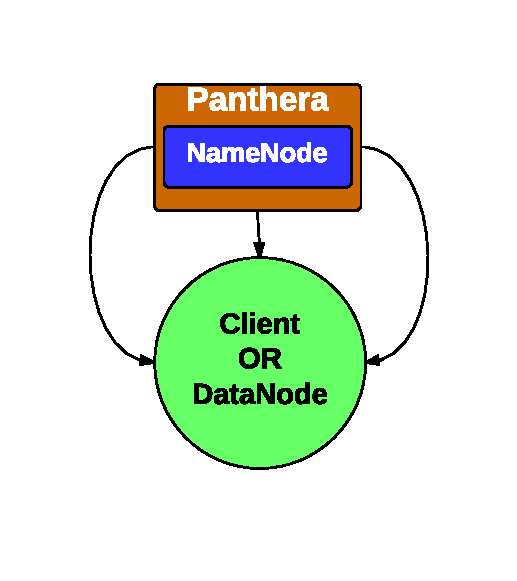
\includegraphics[scale=1.2]{assets/panthera_metadata_large.pdf}}
      	%\end{block}

      
      %\begin{block}{Panthera Data Architecture}
      %\centerline{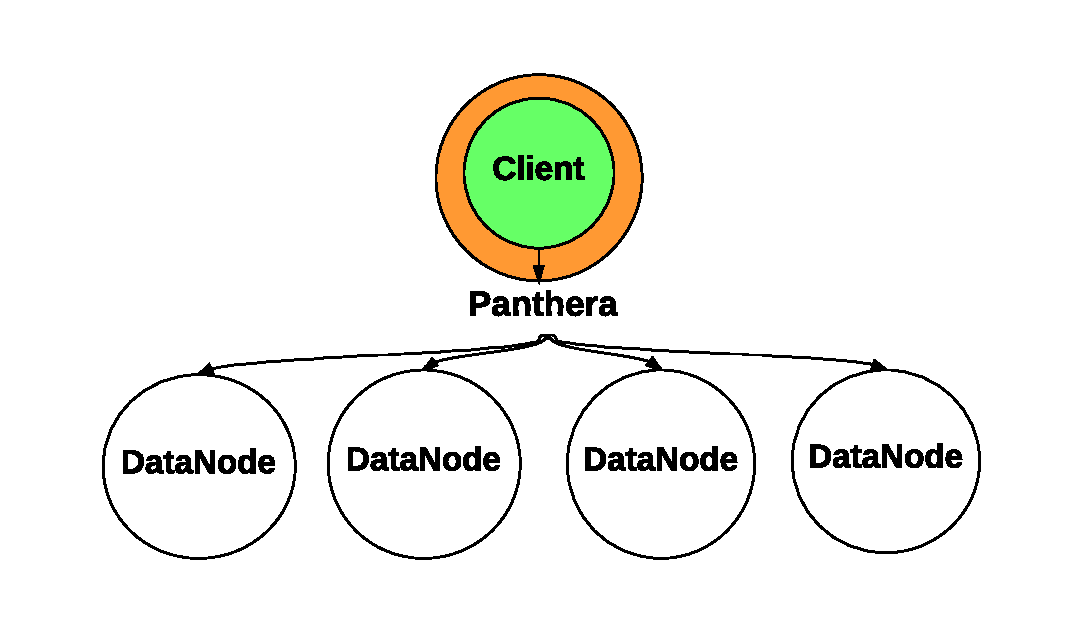
\includegraphics[scale=1.2]{assets/panthera_data_architecture.pdf}}
     %\end{block}

	\begin{block}{Panthera - Implementation}
	\begin{itemize}
		\item \textbf{Panthera is implemented on Google's Go programming language} which has excellent concurrency primitives and memory management, making it perfect for
		for software like \textbf{Panthera} that must run reliably with hundreds of clients.
	\end{itemize}
	\end{block}
	
	\begin{block}{Latency Testing Methodology}
	Client and server (i.e. NameNode or DataNode) are on separate machines
	for both metadata and data cache testing.
	\begin{itemize}
		\item \textbf{Metadata}: Repeatedly request directory listing for a directory with 100 files in it.
		\item \textbf{Data}: Repeatedly request file contents for a 1MB large file.
	\end{itemize}

	\end{block}
		\begin{block}{Latency Results}
		\vspace{1em}
		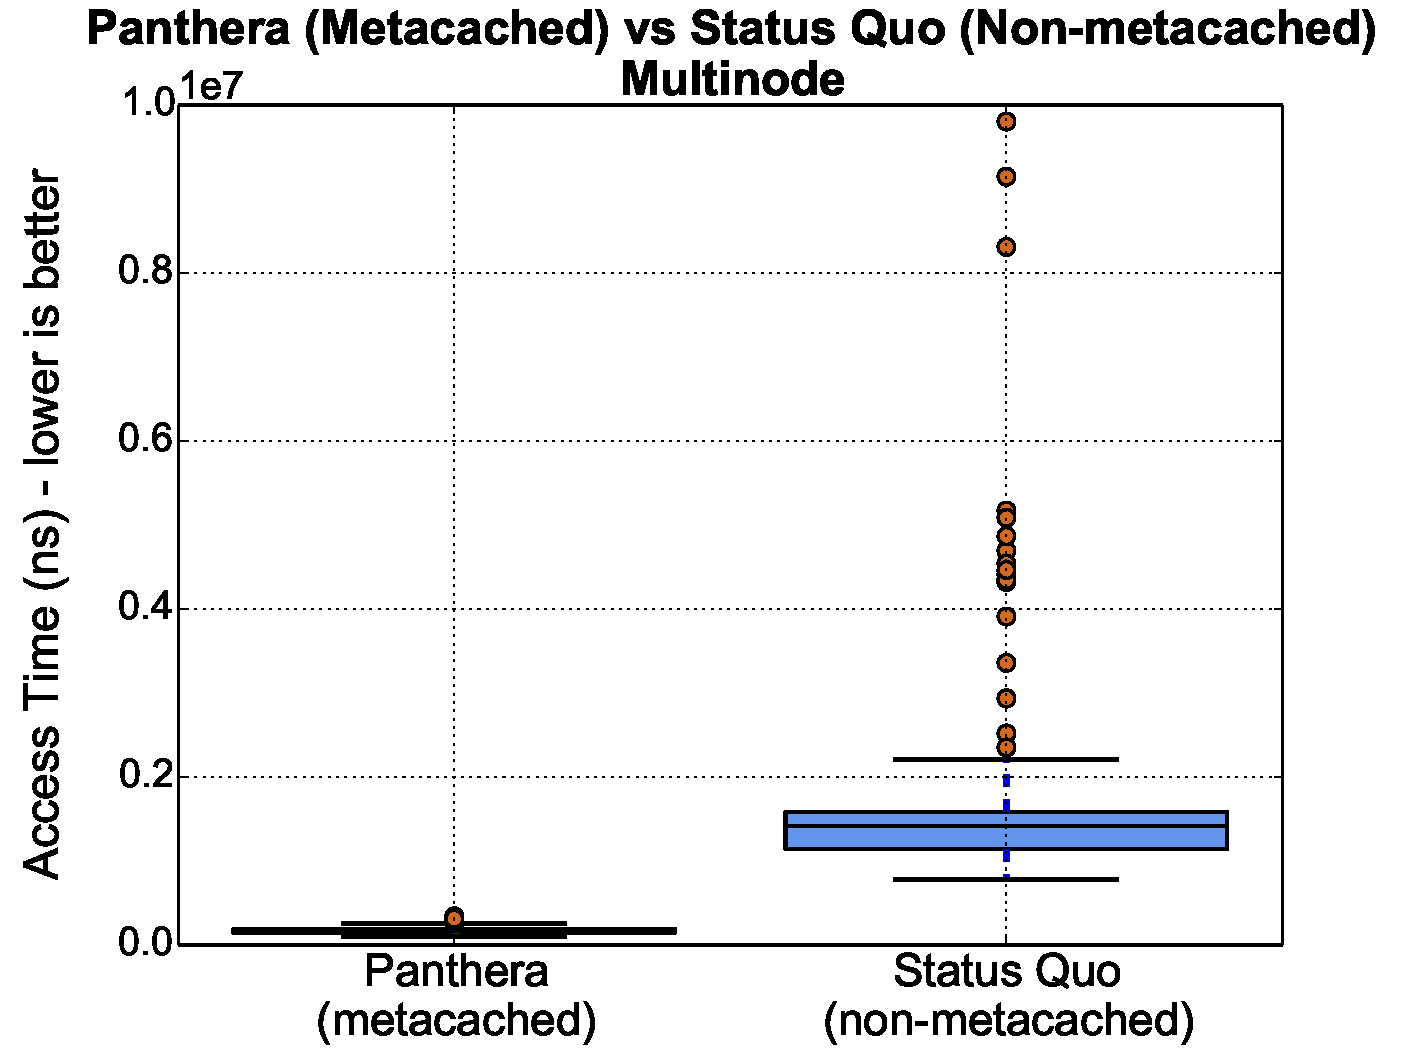
\includegraphics[scale=1]{assets/v2/multinode_meta_box_plot.pdf}
		\vspace{1.5em}
		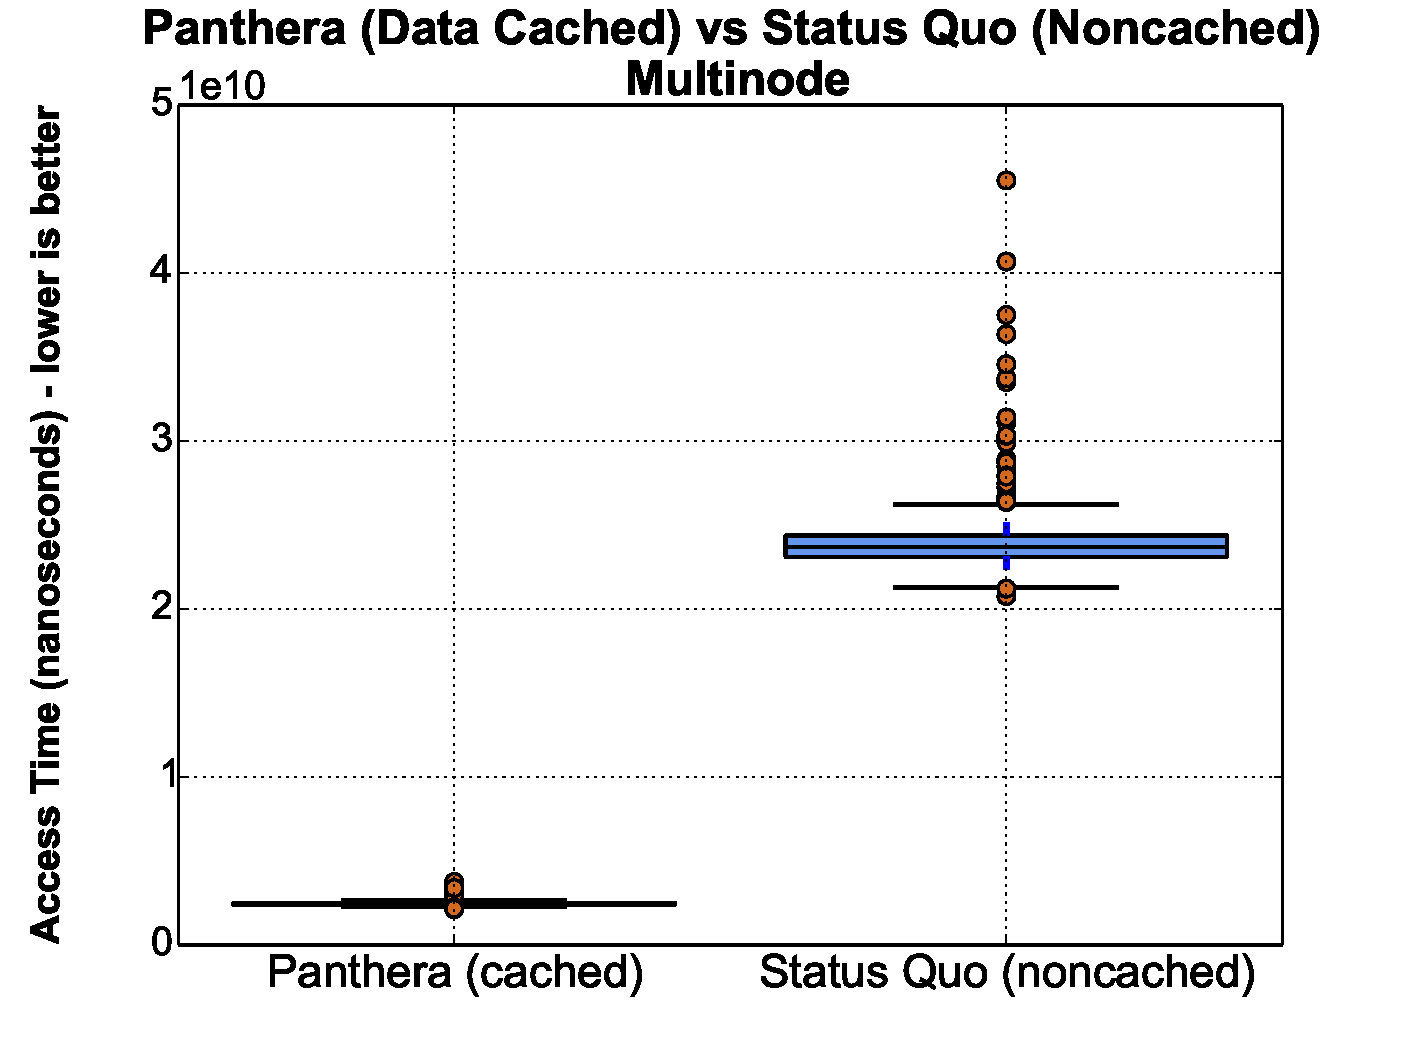
\includegraphics[scale=0.98]{assets/v2/getter_boxplot.pdf}
		%\vspace{1em}
		%\includegraphics[scale=0.98]{assets/v2}
	\end{block}
	
	\begin{block}{Procedure Testing Methodology}
	Panthera was also tested with running times of algorithms running on Hadoop (as opposed to simply downloading files). The input sample was a repeated copyof "The 
	Adventures of Sherlock Holmes" (192 MB).
	\begin{itemize}
	\item \textbf{WordCount}: The classic distributed algorithm that counts occurrences
	of all words in a given text.
	\item \textbf{ReferenceCount}: Counts occurrences of words in a given text, but 
	only considers the words that are in a given reference file (i.e. dictionary).
	\end{itemize}
	\end{block}
	


	  
      \end{column}
      %##########################################################
      
      
      \begin{column}{0.32\textwidth}
		\begin{block}{Procedure Results}
		\vspace{1em}
		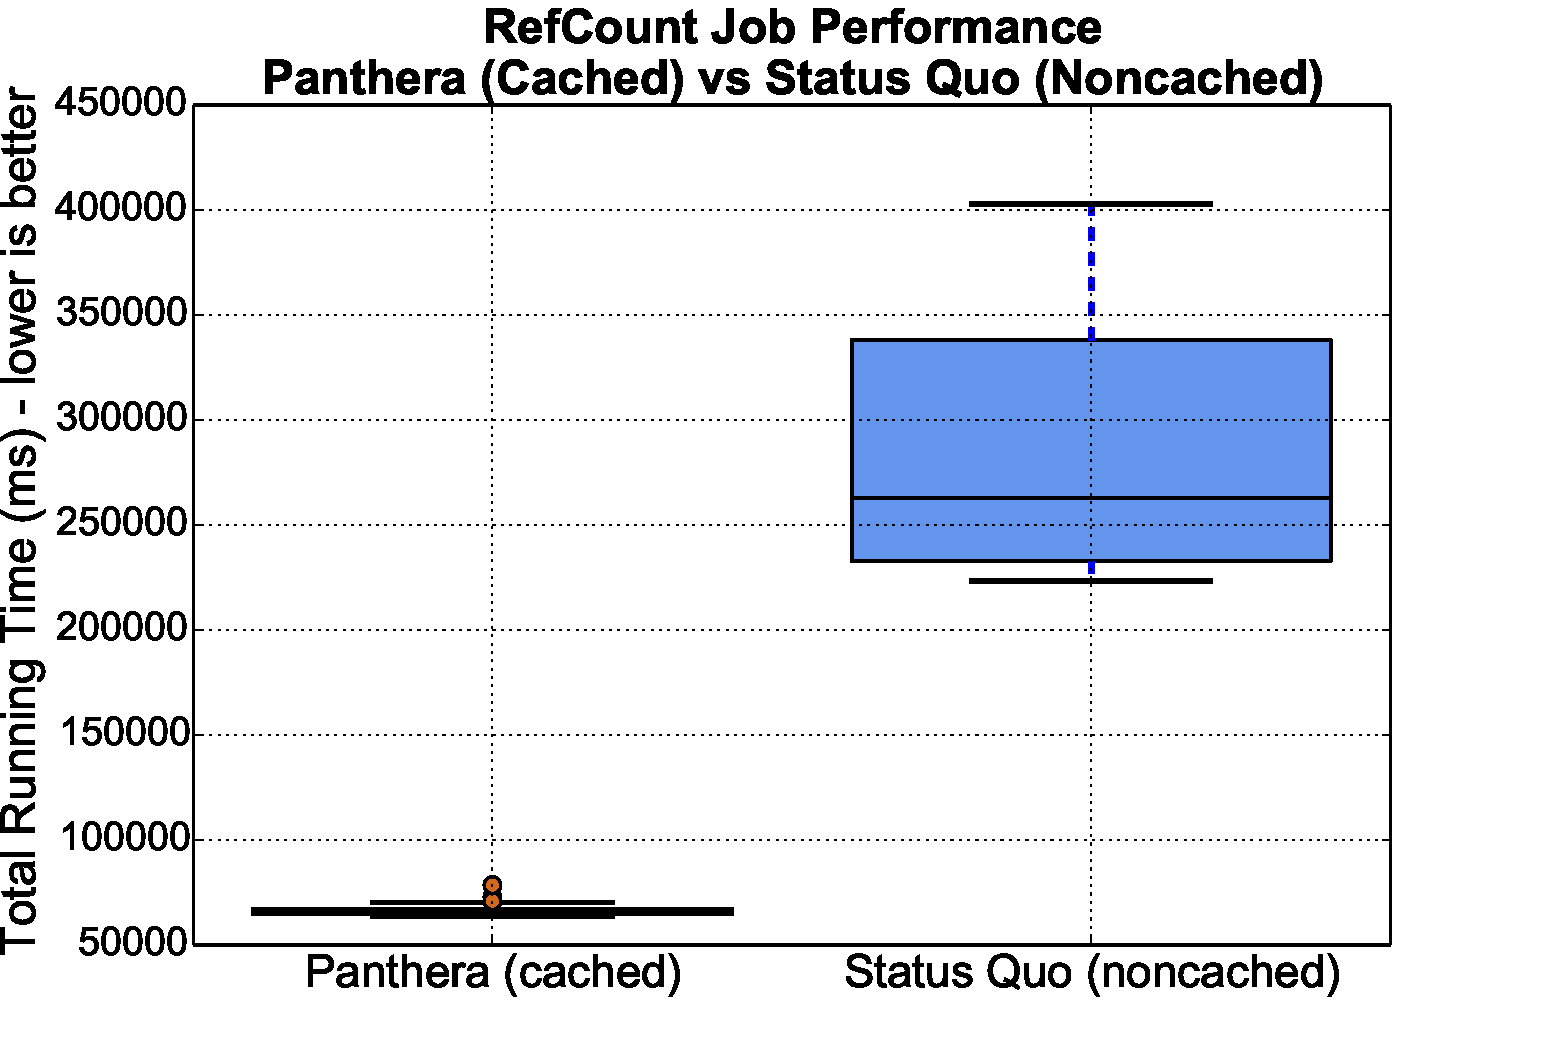
\includegraphics[scale=1]{assets/v2/refgetter_boxplot.pdf}
		\end{block}
	
	  \begin{block}{Latency Types}
		%discuss the types of latency and make the comparison
		%between hard disk latency and regular lateny
		In the Hadoop File System Architecture, there are several types of latency involved (listed from highest to lowest latency):
		\begin{itemize}
		\item \textbf{Network latency}
		\item \textbf{Hard drive latency}
		\item \textbf{Memory latency: } Reading from RAM memory has an extremely small
		waiting time associated with it. \textbf{Panthera converts hard drive latency to memory latency, thereby greatly reducing file access time.}
		\end{itemize}
	  \end{block}
	
	
	
    \begin{block}{Statistics}
	\begin{table}
	\setlength{\tabcolsep}{25pt}
	\centering
	\begin{tabular}{lc}
		\toprule
		\textbf{Type} & \textbf{Mean time improvement} \\
		\midrule
		Metadata   & 862.6\% \\
		Data       & 863.4\% \\
		Word count & \phantom025.1\% \\
		Ref. count & 331.6\% \\
	\bottomrule
	\end{tabular}
	\caption{Improvement with Panthera in the total amount of time required to execute algorithms/requirements (compared with status quo)}
	\end{table}
 	
 	\vspace{1em}
	\begin{table}
	\setlength{\tabcolsep}{25pt}
	\centering
	\begin{tabular}{lc}
		\toprule
		\textbf{Type} & \textbf{Standard deviation contraction} \\
		\midrule
		Metadata   & 27.38x \\
		Data       & 11.14x \\
		Word count &  0.78x \\
		Ref. count & 22.91x \\
	\bottomrule
	\end{tabular}
	\caption{Reduction obtained with Panthera in the standard deviation of running times, i.e. a contraction of 9x implies that the standard deviation was reduced
	by a factor of 9 with Panthera (compared to the status quo).}
	\end{table}

    \end{block}
    
    	\begin{block}{Conclusion}
    	The results validate the hypothesis presented.
    	\begin{itemize}
    		\item Panthera was successfully developed as a "drop-in" solution
    		\item It was able to reduce latency in comparison to a standard Hadoop installation. 
    		\item A scheduler was also implemented which uses cache information to schedule
    		Hadoop jobs.
    		\item Metadata latency was \textbf{decreased by a factor of 7.36}
    		\item Data latency was \textbf{decreased by a factor of 7.634}
    		\item The running of time of WordCount (an algorithm with very few file accesses) was \textbf{improved by 25\%} with the code left unmodified.
		\item The running time of RefCount was \textbf{improved by 331.6\%}.
    	\end{itemize}
	 
    	As a "drop-in" solution, Panthera can be employed in a variety of 
    	applications to improve performance without code modification. With the 
    	demonstrated time and resource savings, Panthera can have incredible 
    	impacts in distributed systems and in specific applications.
	
	\end{block}
	
	\begin{block}{Applications}
	Hadoop has diverse applications and since Panthera was created as a "drop-in" solution, the \textbf{applications span an extremely wide range of disciplines}.
	\begin{itemize}
		\item Bioinformatics (e.g. CrossBow from Johns Hopkins University)
		\item Numerical/scientific computing 
		\item Image processing
		\item Artificial Intelligence/Machine Learning (e.g. Apache Mahout)
		\item Market Research (e.g. Target)
	\end{itemize}
	\end{block}
	
	\begin{block}{Future Work}
	\begin{itemize}
		\item \textbf{All code related to this project will be open sourced} to further development in distributed computing.
		\item Currently working on testing a \textbf{bioinformatics toolkit with Panthera}; initial results are very promising and show significant reduction in total running time.
		\item Smart scheduling using Panthera; arranges tasks so that the cache is used most efficiently.
		
	\end{itemize}
	\end{block}
      \end{column}
    \end{columns}
  \end{frame}
    
  \end{document}